\author{Harrison Deng}

\documentclass[11pt]{article}
\usepackage{fullpage}
\usepackage{amsmath,amsthm,amssymb}
\usepackage{xifthen}%
\usepackage[hidelinks,colorlinks]{hyperref}
\setlength\parindent{0pt}
\usepackage{tikz}
\usepackage{algorithm}
\usepackage{algpseudocode}
\usetikzlibrary{positioning}

% Counter for Questions
\newcounter{question}

% Question
\newcommand{\question}[2]{%
	\stepcounter{question}
	\vspace{.25in} \textbf{Q\arabic{question} 
		\ifthenelse{\isempty{#1}}%
		{}% if no points
		{[#1 Points]\ }% if #1 is not empty
		#2}\vspace{0.10in}
}

% Subquestion
\newcommand{\qpart}[2]{%
	\vspace{.10in} \textbf{(#1)}
	\ifthenelse{\isempty{#2}}%
	{}% if no points
	{[#2 Points]}% if #1 is not empty
}

\newcommand{\references}{\vspace{.25in}\textbf{References}\vspace{.10in}}

% Solution to question
\newcommand{\solution}{\vspace{.25in}\textbf{Solution}\vspace{.10in}}

% Solution to subquestion
\newcommand{\solpart}[1] {\vspace{.10in}\textbf{(#1)}}

% Should the solutions be displayed?
\newif\ifsolutions
\solutionstrue

% Should the marking scheme be displayed?
\newif\ifmarkingscheme
\markingschemefalse

% Math commands
\newcommand{\set}[1]{\{#1\}}
\newcommand{\floor}[1]{\lfloor#1\rfloor}
\newcommand{\ceil}[1]{\lceil#1\rceil}
\DeclareMathOperator*{\argmin}{arg\,min}
\DeclareMathOperator*{\argmax}{arg\,max}

\title{CSC373 Assignment 4 Submission}
\date{\today}
\begin{document}
\maketitle

\question{15}{Set Cover}

Here is the {\it Set-Cover} problem. You are given a set $E = \{ e_1, ..., e_n \}$, and $m$ subsets $S_1, ..., S_m \subseteq E$. For each $j \in [m]$, we associate a weight $w_j \geq 0$ to the set $S_j$. The goal is to find a minimum-weight collection of subsets that covers all of $E$. 

\qpart{a}{5} Form the set-cover problem as an integer linear program, and then relax it to a linear program. Define your variables. [Hint: you might want to have a constraint like $\sum_{j:e_i \in S_j} x_j \geq 1$ for each element $e_i$.]

\qpart{b}{5} Let $x^*$ denote the optimal solution to the relaxed LP you defined in part (a). Let $f$ be the maximum number of subsets in which any element appears. Here's the rounding algorithm: given $x^*$, we include $S_j$ if and only if $x^*_j \geq 1/f$. Let $I = \{ j : S_j \text{ is selected by the rounding algorithm} \}$. Prove that the collection of subsets $S_j$ where $j \in I$ chosen by the rounding algorithm is a set cover.

\qpart{c}{5} Let ${\sf OPT}$ be value of the optimal solution of the set-cover. Prove that the rounding algorithm in (b) gives an $f$-approximation.

\newpage

\question{15}{Traveling Salesman}

Here's the {\it metric traveling salesman} problem. You are given a complete graph $G = (V,E)$, where $V = \{ 1, ..., n \}$ represents the cities the salesman needs to visit. For each edge $(i,j) \in E$, we associate it with a cost $c_{ij}$. We call it ``metric" because for every triplet of vertices $i,j,k \in V$, it respects the triangle inequality, i.e.~$c_{ik} \leq c_{ij} + c_{jk}$. The goal is to have a tour of the cities (i.e. a Hamiltonian cycle of $G$) such that each city is visited exactly once (except for the starting city where you have to come back to), and the total cost is minimized. \\

Here is our approximation algorithm, which is also a greedy algorithm: Among all pairs of cities, find the two closest cities, say $i$ and $j$, and start by building a tour on that pair of cities; the tour consists of going from $i$ to $j$ and then back to $i$ again. This is the first iteration. In each subsequent iteration, we extend the tour on
the current subset $S \subseteq V$ by including one additional city, until we include the full set of cities. Specifically in each iteration, we find a pair of cities $i \in S$ and $j \notin S$ for which the cost $c_{ij}$ is minimum; let $k$ be the city that follows $i$ in the current tour on $S$. We add $j$ to $S$, and replace the path $i\to k$ with $i \to j$ and $j \to k$. See the picture below for illustration:
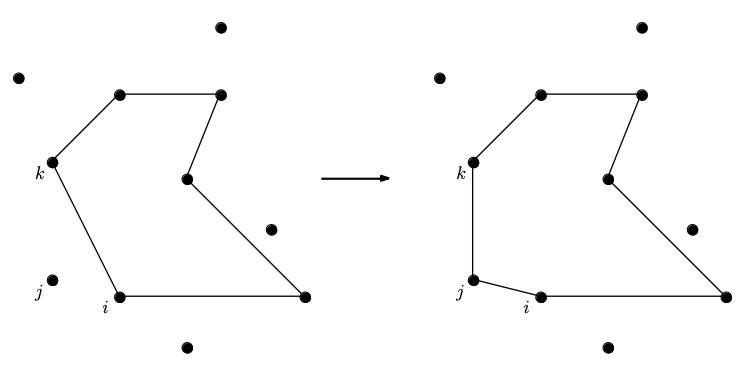
\includegraphics[scale=0.29]{q2_tsp.png}

Let ${\sf OPT}$ be the value of the optimal solution of the metric traveling salesman problem. Prove that the approximation algorithm above gives a 2-approximation.

\solution

\textbf{Variables and Assumptions}: To begin, we will define our variables and state our assumptions, let \(G = (E, V)\) be the complete graph where \(V\) represents the spatial nodes to be visited and \(E\) be a series of edges that connect all vertices with each other. Each edge is assigned a weight \(c_{ij}\) for the corresponding vertices \(i\) and \(j\). Furthermore, we will assume that the triangle inequality holds for all triangles formed by all edges. In other words, \(\forall i, j, k \in V, c_{ik} \leq c_{ij} + c_{jk}\) essentially stating that for any given vertices \(i\), \(j\), \(k\), the direct edge from \(i\) to \(k\) is never worse than the sequence of edges from \(i\) to \(j\), to \(k\). Let \verb|GRD| be the described greedy algorithm given in the question. We let function \(c(S)\) be the sum of all edge weights for traversing all vertices of a graph \(S\). Lastly, we will assume \verb|OPT| the cost of the a optimal solution to traveling salesman problem (TSP). Our objective is to show that, given \(S_g\) solution generated by \verb|GRD| \(S_g\) is at worst, \(c(S_g) \leq 2 \times \verb|OPT|\).

\medskip

\textbf{Claim 1}: To begin, notice that the \(c(S_o)\) such that \(c(S_o) = \verb|OPT|\), is a cycle that traverses all vertices minimally and cyclically where each node is traversed exactly once with the exception of the starting node. Then, see that \(c(S_o)\) may be trivially converted into a tree graph by simply removing any edge in \(S_o\) and arbitrarily selecting a vertex to become the root of the tree. Furthermore, see that the traversal of such a tree costs will not cost more than the traversal of the original cycle \(S_o\). In other words, \(S_o = (E_o, V_o), \forall e \in E_o, c(S_o - \{e\}) \leq c(S_o)\).

% TODO Double check if the definition of the w function makes sense.

\medskip

\textbf{Prim's Minimum Spanning Tree Algorithm Review}: Very briefly,the Prim's minimum spanning tree (MST) algorithm begins by arbitrarily selecting a vertex from a graph, and iteratively selecting the next vertex with the lowest edge weight connecting to the current set of selected vertices.

\medskip

\textbf{Claim 2}: See that the cycle graph \(S_e = (E_e, V_e)\) generated by \verb|GRD| will always result in requiring half of the edges to traverse all nodes via connected edges when compared to traversing a MST. To see this, we assert that \verb|GRD| produces a traversal graph (vertices representing nodes and edges representing the edge taken to reach each vertex) \(S_g = (E_g, V_g)\) that is no different from a graph produced by Prim's MST algorithm \(S_p = (E_p, V_p)\) from \(G\), after running a depth first search (DFS) on \(S_p\), and removing the duplicates, connecting edges that traversed to the duplicate vertices directly to the subsequent vertex after the removed vertex.

\smallskip

This is because \verb|GRD| is substantially different only in the step of adding the selected vertex to the current graph. Where in Prim's, the algorithm selects the vertex \(s \in G\) associated with the lowest weighted edge that connects to a vertex \(i\) in the partial solution \(S_{pp} = (E_{pp}, V_{pp})\) and proceeding to the next iteration, \verb|GRD| selects the next vertex and edge identically, however, instead of moving to the next iteration, \verb|GRD| connects \(s \in G\) to the next node \(i\) is linked to \(k \in S_{pp}\). In other words, where Prim's may resolve to connect \(i \rightleftarrows s\) such that \( E_{pp} = \{\ldots, \{i, k\}, \{i, s\}, \ldots\} \), and a traversal by DFS results in a sequence \(\ldots \rightarrow i \rightarrow k \rightarrow i \rightarrow s \rightarrow \ldots \). \verb|GRD| resolves the newly selected vertex such that \( E_{pp} = \{\ldots, \{i, s\}, \{s, k\}, \ldots\} \), effectively changing \(i \rightleftarrows k\) to \(i \rightleftarrows s \rightleftarrows k \) where the traversal is trivially \( \ldots \rightarrow i \rightarrow s \rightarrow k \rightarrow \ldots \) thus maintaining the chain form of the graph. From this breakdown, we can see that the Prim's approach requires double the edges for the full traversal in contrast against the \verb|GRD| algorithm. 

\smallskip

However, to see that the methods are analogous and thus, comparable, the DFS traversal \(\ldots \rightarrow i \rightarrow k \rightarrow i \rightarrow s\ \rightarrow \ldots \) can be simplified into \(i \rightarrow k \rightarrow s\) (removing the second appearance of \(i\) in the sequence) without worsening the total weight required for the traversal by the triangle inequality (TI) assumption. To prove this, we may focus on \(k \rightarrow i \rightarrow s\), and see that \(c_{ks} \leq c_{ki} + c_{is}\) (TI assumption).

\smallskip

From this, we can see that Prim's algorithm is known to generate a MST, and to traverse such a tree in it's entirety is double the cost of the cyclical traversal path provided by \verb|GRD|. In other words, we have proven \(2 c(S_p) = (c(S_g))\) or \(c(S_p) = \frac{1}{2}(c(S_g))\).

\medskip

\textbf{Proof of 2-Approximation}:

\begin{align}
	c(S_p) &\leq c(S_o - \{e\}) &(\text{Prim's Algorithm generates MST}) \\
	\frac{1}{2} c(S_g) &\leq c(S_o - \{e\}) &(\text{Claim 2}) \\
	\frac{1}{2} c(S_g) &\leq c(S_o - \{e\}) \leq c(S_o) &(\text{Claim 1}) \\
	c(S_g) &\leq 2c(S_o)
\end{align}

Where \(S_g\) is the solution produced by \verb|GRD|, and \(S_o\) is the optimal solution. Hence, we've shown that the described \verb|GRD| algorithm will always result in a solution no worse than twice the optimal solution, i.e., 2-approximation.

\newpage

\question{20}{Randomized Algorithms}

Let $G = (V,E)$ be an undirected graph. For any subset of vertices $U \subseteq V$, define
\[
    {\sf cut}(U) = \{ (u,v) \in E : u \in U \text{ and } v \notin U \}.
\]
The set ${\sf cut}(U)$ is called the {\it cut} determined by the vertex set $U$. The size of the cut is denoted by $|{\sf cut}(U)|$. The {\it Max-Cut} problem asks you to find the cut with maximum size, i.e., $\max_{U \subseteq V} |{\sf cut}(U)|$. \\

Here is a randomized algorithm for {\it Max-Cut}: Take a uniform random subset $U$ of $V$, and choose ${\sf cut}(U)$ to be the cut. Let {\sf OPT} be the size of the maximum cut in $G$. Prove that the randomized algorithm gives a cut of expected size at least half of the optimal solution, i.e.,~$\mathbb{E}[|{\sf cut}(U)|] \geq \frac{1}{2}{\sf OPT}$. 

\newpage

\question{5}{Extra Credit}

``Here is the link for EC3, you should submit this with HW4 (not HW3)." --- Harry\\

\url{https://colab.research.google.com/drive/1Mo8S-asikkd4qBakMldCwlsDHcpyzEmo?usp=sharing}

\vspace{\baselineskip}
\references \\
Please write down your references here, including any paper or online resources you consult.

\end{document}